\documentclass[11pt]{amsart}
\usepackage[T1]{fontenc}
\usepackage{lmodern}
\usepackage[margin=1.1in]{geometry}
\usepackage{amssymb,amsmath,mathtools}
\usepackage{booktabs}
\usepackage[hidelinks,hypertexnames=false]{hyperref}
\usepackage{xcolor}
\usepackage{tikz}
\usetikzlibrary{arrows.meta,calc,positioning}
% Okabe--Ito colors used by the figures
\definecolor{pA}{HTML}{0072B2}\definecolor{pB}{HTML}{E69F00}\definecolor{pC}{HTML}{009E73}\definecolor{pD}{HTML}{CC79A7}
\setlength{\emergencystretch}{1.5em}

\newtheorem{theorem}{Theorem}[section]
\newtheorem{proposition}[theorem]{Proposition}
\newtheorem{lemma}[theorem]{Lemma}
\theoremstyle{remark}
\newtheorem{remark}[theorem]{Remark}

\newcommand{\F}{\mathbb{F}}
\DeclareMathOperator{\srg}{srg}
\DeclareMathOperator{\Aut}{Aut}
\DeclareMathOperator{\AGL}{AGL}
\DeclareMathOperator{\GL}{GL}

\title[Strongly regular graphs on 400 vertices]{Strongly regular graphs with parameters $(400,168,68,72)$}
\author{Dylan Plummer}
\date{25 November 2026}

\begin{document}

\begin{abstract}
Brouwer's table lists the parameters $(400,168,68,72)$ as open. We construct about $5.4\cdot10^{122}$ pairwise non-isomorphic strongly regular graphs with these parameters and count them exactly. There are twelve decompositions of the complement of the Hoffman--Singleton graph into $35$ copies of the triangular graph $T(5)$ invariant under the same group $C_5\times C_5$, each given by three base blocks. Every point is replaced by $\F_2^3$, the seven tiles at a point receive the seven nonzero characters, and each tile is signed by the roots of $A_4$. The proof uses a lifting lemma for edge decompositions into signed graphs with two eigenvalues, and it settles a case that A.~Kova\v{l}'s hyperplane-slab template left open. The fibers can be recovered from the graph, which gives the count. Reversing the signs on $30$ of the $35$ tiles gives a bijection with the same number of graphs with the known parameters $(400,171,74,72)$. No graph in the family is the point graph of a partial geometry $pg(14,11,6)$. Up to $1300$ vertices, we list the other open rows that the lemma reaches by arithmetic. A companion note uses the same local rule to construct $\srg(496,231,102,112)$.
\end{abstract}

\maketitle

\section{Introduction}

Section~\ref{sec:lemma} proves a lifting lemma: a regular graph whose edges are split into signed tiles with two eigenvalues lifts to a strongly regular graph on $F$ times as many vertices, for any Hadamard matrix of order $F$. Section~\ref{sec:construction} applies it to the complement of the Hoffman--Singleton graph with $F=8$. Section~\ref{sec:family} counts the resulting graphs, Section~\ref{sec:covers} adds eleven further tilings and a companion family with parameters $(400,171,74,72)$, and Section~\ref{sec:other} lists the other open rows the lemma could reach. Figure~\ref{fig:flow} shows which results rest on computations.

The same local rule gives $\srg(496,231,102,112)$ in a companion note~\cite{P496}. There the tiles are copies of $T(6)$ signed by the roots of $A_5$, and they decompose the complete multipartite graph $K_{15\times4}$. That base graph does not satisfy the hypothesis of Lemma~\ref{lem:lift}, so the lift is made at the level of an equiangular tight frame: one coordinate per part ties together the fibers of a part, and an extra fiber of $16$ vectors at an added point makes the frame tight. This gives a regular two-graph, and a switching gives the graph. Both constructions lead to the same open rows on $616$ vertices (Section~\ref{sec:other}).

\section{A lifting lemma}\label{sec:lemma}

Let $B$ be a graph on a set $P$ of $v$ points. A \emph{tile} is a set $V_T\subseteq P$ with a symmetric matrix $X_T$ on $V_T$ with entries $0,\pm1$ and zero diagonal. A \emph{tiling} of $B$ is a set of tiles whose nonzero entries partition the edges of $B$. Let $H$ be a Hadamard matrix of order $F$ whose first row is all ones, and let $h_2,\dots,h_F$ be its other rows. Suppose every point lies in exactly $F-1$ tiles. At each point $p$ choose a bijection from its tiles to $\{2,\dots,F\}$ and a sign for each tile, and let $f_{p,T}=\pm h_i$ be the resulting row. Fix $c\in\{0,1\}$.

The graph $\Gamma$ has vertex set $P\times\{1,\dots,F\}$; we call $\{p\}\times\{1,\dots,F\}$ the \emph{fiber} of $p$. Two vertices in one fiber are adjacent if and only if $c=1$. Two vertices $(p,x)$ and $(q,y)$ with $p\ne q$ are adjacent if and only if $pq$ is an edge of $B$ in the tile $T$ and
\[
f_{p,T}(x)\,f_{q,T}(y)=X_T(p,q).
\]
So every vertex has $F/2$ neighbors in each neighboring fiber (Figure~\ref{fig:lift}).

\begin{lemma}\label{lem:lift}
Suppose $B$ is regular of degree $k_B$ with eigenvalues $\theta_1,\theta_2$ on the complement of the all-ones vector, and every $X_T$ has eigenvalues in $\{\theta_1+2c,\theta_2+2c\}$. Then $\Gamma$ is regular of degree $c(F-1)+Fk_B/2$, and its other eigenvalues are $F(\theta_1+2c)/2-c$ and $F(\theta_2+2c)/2-c$. In particular $\Gamma$ is strongly regular when $B$ is connected and these two numbers are distinct.
\end{lemma}

\begin{proof}
Let $A$ be the adjacency matrix of $\Gamma$. On functions that are constant on fibers, $A$ acts as $c(F-1)I+\tfrac F2A_B$, because the rows $f_{p,T}$ are orthogonal to the all-ones vector. For a tile $T$, let $W_T$ be the space of functions that are supported on the fibers of $V_T$ and equal $a_pf_{p,T}$ on the fiber of $p$, for $a\in\mathbb R^{V_T}$. At a point shared by two tiles the two vectors $f_{p,T}$ are different rows of $H$ up to sign, so the spaces $W_T$ are orthogonal to each other and to the fiber-constant functions. Their dimensions add up to $v+v(F-1)=Fv$, so together they span everything.

Take $g=a_qf_{q,T}$ on the fiber of $q$. The block of $A$ between the fibers of $p$ and $q$ is $\tfrac12\bigl(J+X_{T'}(p,q)f_{p,T'}f_{q,T'}^{\top}\bigr)$, where $T'$ is the tile of $pq$. It sends $g$ to $\tfrac F2X_T(p,q)a_qf_{p,T}$ if $T'=T$ and to $0$ otherwise. Inside a fiber, $c(J-I)$ sends $f_{q,T}$ to $-cf_{q,T}$. Hence $A$ acts on $W_T$ as $-cI+\tfrac F2X_T$, with the two stated eigenvalues. On the fiber-constant functions orthogonal to the all-ones vector the eigenvalues are $c(F-1)+\tfrac F2\theta_i=\tfrac F2(\theta_i+2c)-c$, the same two numbers.
\end{proof}

Write $\rho=\theta_1+2c$ and $\sigma=\theta_2+2c$. The diagonal of $X_T^2=(\rho+\sigma)X_T-\rho\sigma I$ shows that every tile has degree $-\rho\sigma$ at each of its points. Since every point lies in $F-1$ tiles, $k_B=(F-1)(-\rho\sigma)$. Section~\ref{sec:other} uses this to find targets.

\begin{remark}
With $c=0$, $B=K_v$ and all-positive cliques as tiles ($\sigma=-1$), the tiling is a Steiner $2$-design with replication number $F-1$, and the lemma gives the constructions of Wallis~\cite{Wal71} and Fon-Der-Flaass~\cite{FDF02}; see also Muzychuk~\cite{Muz07}. Kova\v{l}'s hyperplane-slab template~\cite{Kov26} uses fibers $\F_q^N$ with slab blocks, and its binary case is the case of a Sylvester matrix $H$ here. The lemma allows any Hadamard order and any signed tiles with two eigenvalues. Examples are the signed Johnson graphs $jI-D^{\top}D$, where $D$ is the oriented boundary matrix from $j$-subsets to $(j-1)$-subsets of an $m$-set, with eigenvalues $j$ and $j-m$, and more generally $2I-RR^{\top}$ for a set $R$ of roots that forms a tight frame.
\end{remark}

\begin{figure}[t]
\centering
% Figure 1: (a) the oriented K5 behind the signed tile, (b) the block between two fibers.
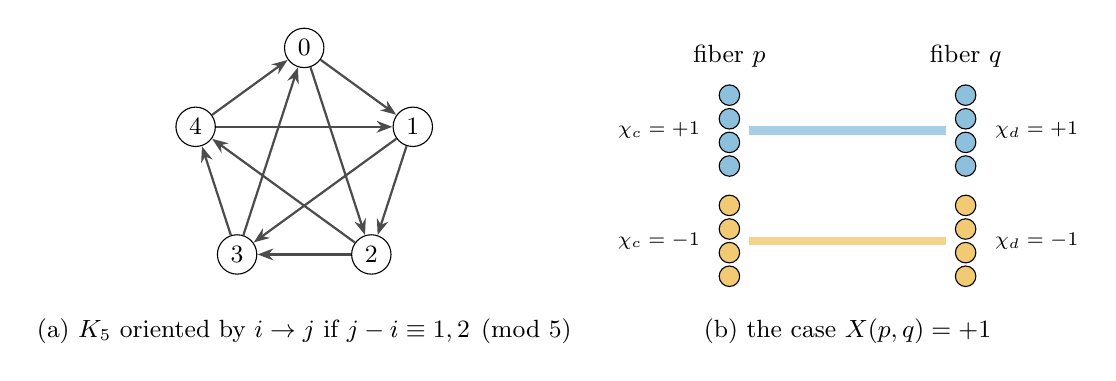
\begin{tikzpicture}[font=\small,
  sym/.style={circle, draw, inner sep=1.5pt, minimum size=5mm, fill=white},
  v/.style={circle, draw, inner sep=0pt, minimum size=2.6mm},
  vp/.style={v, fill=pA!45},
  vm/.style={v, fill=pB!55},
  arc/.style={-{Stealth[length=2mm]}, thick, gray!60!black}]
% ---- (a) K5 oriented by i -> j iff j - i = 1, 2 mod 5
\begin{scope}
  \foreach \i in {0,...,4} \coordinate (k\i) at (90-72*\i:1.45);
  \foreach \i in {0,...,4} {
    \pgfmathtruncatemacro{\j}{mod(\i+1,5)}\pgfmathtruncatemacro{\l}{mod(\i+2,5)}
    \draw[arc, shorten >=2.6mm, shorten <=2.6mm] (k\i) -- (k\j);
    \draw[arc, shorten >=2.6mm, shorten <=2.6mm] (k\i) -- (k\l);}
  \foreach \i in {0,...,4} \node[sym] at (k\i) {\i};
  \node[align=center] at (0,-2.15) {(a) $K_5$ oriented by $i\to j$ if $j-i\equiv1,2\pmod5$};
\end{scope}
% ---- (b) block between fibers p and q
\begin{scope}[xshift=5.4cm, yshift=-0.2cm]
  \node at (0,1.55) {fiber $p$};
  \node at (3,1.55) {fiber $q$};
  \foreach \k in {0,...,3} \node[vp] (a\k) at (0,1.05-0.3*\k) {};
  \foreach \k in {0,...,3} \node[vm] (b\k) at (0,-0.35-0.3*\k) {};
  \foreach \k in {0,...,3} \node[vp] (c\k) at (3,1.05-0.3*\k) {};
  \foreach \k in {0,...,3} \node[vm] (d\k) at (3,-0.35-0.3*\k) {};
  \draw[pA, line width=3pt, opacity=0.35] (0.25,0.6) -- (2.75,0.6);
  \draw[pB, line width=3pt, opacity=0.45] (0.25,-0.8) -- (2.75,-0.8);
  \node[font=\scriptsize, anchor=east] at (-0.25,0.6) {$\chi_c=+1$};
  \node[font=\scriptsize, anchor=east] at (-0.25,-0.8) {$\chi_c=-1$};
  \node[font=\scriptsize, anchor=west] at (3.25,0.6) {$\chi_d=+1$};
  \node[font=\scriptsize, anchor=west] at (3.25,-0.8) {$\chi_d=-1$};
  \node[align=center, font=\small] at (1.5,-1.95) {(b) the case $X(p,q)=+1$};
\end{scope}
\end{tikzpicture}

\caption{(a) The orientation of $K_5$ that signs the tiles of Section~\ref{sec:construction}. (b) The block of $\Gamma$ between the fibers of two points $p,q$ of a tile, when $X(p,q)=+1$ and the tile has characters $\chi_c$ at $p$ and $\chi_d$ at $q$. Each fiber splits into the halves where its character is $+1$ (blue) and $-1$ (orange), and equal halves are completely joined. When $X(p,q)=-1$, opposite halves are joined.}
\label{fig:lift}
\end{figure}

\section{The construction}\label{sec:construction}

Take two copies $P,Q$ of $\F_5^2$, with points $P(i,j)$ and $Q(i,j)$ numbered $5i+j$ and $25+5i+j$. Inside $P$, join $P(i,j)$ to $P(i,j\pm1)$. Inside $Q$, join $Q(i,j)$ to $Q(i,j\pm2)$. Join $P(i,j)$ to $Q(u,w)$ if and only if $w-j=-3(u-i)^2$. The result is the Hoffman--Singleton graph $\srg(50,7,0,1)$~\cite{HS60}, and the $25$ simultaneous translations of $P$ and $Q$ act on it. Indeed, two points in the same row of one sheet lie in a pentagon or pentagram and have no common neighbor in the other sheet. Two points in different rows of one sheet have exactly one common neighbor in the other sheet, because the difference of their two quadratic conditions is linear. For a pair across the sheets, the value $w-j+3(u-i)^2$ determines the common neighbors. Let $B$ be the complement. It has degree $42$, eigenvalues $42$, $2$ (multiplicity $21$) and $-3$ (multiplicity $28$), and $1050$ edges.

Number the edges of $K_5$ as $01,02,03,04,12,13,14,23,24,34$, and assign to them, in this order, the points in each row below:
\[
\begin{array}{rrrrrrrrrr}
25&47&41&37&43&35&34&31&28&49\\
25&6&9&29&26&7&5&27&8&28\\
15&41&29&0&48&34&6&19&11&23
\end{array}
\]
Orient $K_5$ by $i\to j$ if $j-i\equiv1,2\pmod 5$ (Figure~\ref{fig:lift}(a)), let $D$ be its $5\times10$ signed incidence matrix, and put $X=2I-D^{\top}D$. The columns of $D$ are roots $e_i-e_j$ of $A_4$, and $X$ is a signing of $T(5)$. Since $DD^{\top}=5I-J$, $X$ has eigenvalues $2$ (multiplicity $6$) and $-3$ (multiplicity $4$). Each row with $X$ is a tile. Under the translations the three tiles have orbits of lengths $5$, $5$ and $25$, which gives $35$ signed copies of $T(5)$. The stabilizers of the two short tiles rotate $K_5$ and preserve the orientation, so the signs on the translated tiles are well defined.

\begin{proposition}\label{prop:tiling}
The $35$ tiles partition the edges of $B$, and every point lies in exactly $7$ tiles.
\end{proposition}

\begin{proof}
For a pair in one sheet, record the smaller of the difference vector and its negative. For a pair across the sheets, record $Q$ minus $P$. The edges of $B$ have $11$ such differences within $P$, $11$ within $Q$ and $20$ across. Each tile edge has a trivial stabilizer, so a short tile covers each of its differences $5$ times and the long tile covers each of its differences once:
\begin{center}\small
\begin{tabular}{llp{0.2\textwidth}p{0.36\textwidth}}
\toprule
tile & $PP$ & $QQ$ & $PQ$\\
\midrule
$1$ ($5$ copies) & -- & $11,13,14,$ $20,22,24$ & -- \\
$2$ ($5$ copies) & $02$ & $01$ & $40,41,43,44$ \\
$3$ ($25$ copies) & $10..14,20..24$ & $10,12,21,23$ & $01,\dots,04,$ $10,11,13,14,$ $20,21,22,24,$ $30,31,32,34$ \\
\bottomrule
\end{tabular}
\end{center}
Every difference of $B$ occurs exactly once in the table, so the $35\cdot30=1050$ tile edges are exactly the edges of $B$. A point has degree $42$ in $B$ and degree $6$ in each of its tiles, so it lies in $7$ tiles.
\end{proof}

\begin{theorem}\label{thm:main}
Take $c=0$, $F=8$, the Sylvester matrix of order $8$ (whose rows other than the first are the nonzero characters of $\F_2^3$), the tiling of Proposition~\ref{prop:tiling}, and any bijections and signs. The resulting graph is strongly regular with parameters $(400,168,68,72)$ and eigenvalues $168$, $8$ (multiplicity $231$) and $-12$ (multiplicity $168$). Its complement has parameters $(400,231,134,132)$.
\end{theorem}

\begin{proof}
Apply Lemma~\ref{lem:lift} with $\theta_1=2$ and $\theta_2=-3$. The degree is $4\cdot42=168$, and the other eigenvalues are $4\cdot2=8$ and $4\cdot(-3)=-12$, so $A^2=96I-4A+72J$.
\end{proof}

The two exported graphs use the following choices. At each sheet origin ($0$ and $25$) the seven tiles are sorted by their lists of unordered pairs, and the $c$-th tile receives the character $x\mapsto(-1)^{c\cdot x}$, with all signs $+1$. This is transported by the translations. The second graph exchanges characters $1$ and $2$ at point $0$ only.
\begin{center}\small
\begin{tabular}{lccc}
\toprule
graph & $|\Aut|$ & $4$-cliques & clique number\\
\midrule
translation-invariant & $25$ & $4{,}958{,}400$ & $10$\\
swap at point $0$ & $1$ & $4{,}958{,}208$ & $10$\\
\bottomrule
\end{tabular}
\end{center}

\section{The family}\label{sec:family}

Theorem~\ref{thm:main} holds for all $(7!)^{50}\cdot2^{350}$ choices of characters and signs. Changing the sign at one point of a tile conjugates $X_T$ by a diagonal sign matrix, which does not change its eigenvalues.

\begin{proposition}[finite check]\label{prop:fibers}
In every member, a set of four distinct vertices whose adjacency rows sum to zero over $\F_2$ is an affine plane inside one fiber. Hence the fibers, the graph $B$ and the tiles are determined by $\Gamma$, and every isomorphism between members maps fibers to fibers.
\end{proposition}

\begin{proof}
On the fiber of a point $q$ adjacent to $p$, the row of $(p,x)$ is an affine function of $y\in\F_2^3$ whose linear part is the character at $q$ of the tile of $pq$. Let $S$ be the set of points used an odd number of times by the four vertices. If $|S|$ is $2$ or $4$, the linear part on the fiber of $q$ is the sum of the characters of the tiles at $q$ that contain an odd number of points of $S$ adjacent to $q$. A finite check (\texttt{family/structure.py}) over all $1225$ pairs and $230{,}300$ sets of four points finds, for each, a point $q$ with exactly one or two such tiles, and one or two distinct nonzero characters never sum to zero. If $S$ is empty, two vertices at $p$ that differ by $d\ne0$ have a row sum equal to the indicator of the fibers reached through the four tiles at $p$ whose character is $-1$ at $d$. The $1750$ resulting supports are pairwise distinct, so two pairs at different points cannot cancel. Four vertices at one point cancel if and only if their coordinates sum to zero.

So two vertices lie in the same fiber exactly when they lie in a common zero-sum set of four. The tiles at $p$ are the classes of neighboring fibers that split the fiber of $p$ in the same way, joined along each connected $T(5)$.
\end{proof}

The automorphisms of $B$ that preserve the tiling form the cover group, of order $50$, isomorphic to $C_5\times D_{10}$, with two orbits of length $25$ on points. So no member is vertex-transitive. An isomorphism between members is an element of the cover group composed with an element of $\AGL(3,2)$ on each fiber. There are $(7!)^{50}\cdot2^{350-35}$ labeled graphs, because the characters are recovered from the splits and the signs are recovered up to reversing a whole tile.

\begin{theorem}\label{thm:count}
The tiling of Proposition~\ref{prop:tiling} gives exactly
\[
N=\tfrac1{50}\bigl(2^{215}15^{50}+5\cdot2^{121}15^{20}61^2+8\cdot2^{39}15^{10}+16\cdot2^{43}15^{10}+20\cdot2^{25}15^{4}\bigr)\approx6.7149\cdot10^{121}
\]
pairwise non-isomorphic strongly regular graphs with parameters $(400,168,68,72)$, and $N\ge30^{50}\cdot2^{165}/50$.
\end{theorem}

The decimal value of $N$ is in \texttt{family/COUNT.txt}. The lower bound divides the number of labeled graphs by $50\cdot|\AGL(3,2)|^{50}$. For the exact value, each fiber carries one of $480$ local states, an affine coset of one of the $30$ labeled $[7,3,4]$ simplex codes formed by its eight sign words. The only other equivalences are the $2^{35}$ tile reversals, which act freely, so there are $480^{50}/2^{35}=2^{215}15^{50}$ classes up to the identity of $B$. Burnside's lemma over the cover group gives the five terms, for elements of orders $1,2,5,5,10$ (\texttt{family/full\_count.py}). A second computation over all $20$ subgroups (\texttt{family/stabilizers.py}) gives the distribution of full automorphism groups. The orders $1,2,5,10,25,50$ all occur, and only a fraction of about $9.8\cdot10^{-60}$ of the graphs have a nontrivial automorphism. The distribution satisfies the orbit--stabilizer identity $\sum_i a_i\cdot50/|G_i|=2^{215}15^{50}$ exactly.

\subsection*{Translation-invariant members}
Choices transported from the two sheet origins give $30^2\cdot2^5=28{,}800$ classes up to the identity of $B$. Here $30=7!/|\GL(3,2)|$, and $2^5$ counts the invariant signs modulo translations within fibers and tile reversals. The involution of the cover group pairs them up, with $512$ fixed points. So there are exactly $14{,}656$ classes: $14{,}144$ with automorphism group $C_5\times C_5$ and $512$ with $C_5\times D_{10}$. We confirmed this count by computing nauty canonical forms for all $14{,}656$ graphs and checking every one on all pairs. As a further check, the $900$ sign-free translation-invariant choices give $888$ classes, $12$ of them with $50$ automorphisms, in agreement with the catalogue.

\subsection*{Cliques}
A clique of $\Gamma$ meets each fiber at most once and projects to a clique of $B$. Inside a tile, three edges of $K_5$ through a common vertex form a triangle of $X$ with sign product $-1$. A lifted triangle has sign product $+1$, because each character value occurs twice, and switching does not change this. So a projected clique cannot contain such a triple. Two independent enumerations of the cliques of $B$ meeting each of the $175$ stars in at most two points found
\[
1,\ 50,\ 1050,\ 11550,\ 68650,\ 210450,\ 302300,\ 179300,\ 39425,\ 2850,\ 95
\]
cliques of sizes $0,\dots,10$, and none larger.

\begin{proposition}[computational]
Every member has clique number at most $10$. In particular no member is the point graph of a $pg(14,11,6)$, whose lines would be cliques of size $15$.
\end{proposition}

In the translation-invariant catalogue the clique numbers $8,9,10$ occur $29$, $227$ and $14{,}400$ times. The existence of $pg(14,11,6)$ remains open.

\section{Twelve covers and the parameters \texorpdfstring{$(400,171,74,72)$}{(400,171,74,72)}}\label{sec:covers}

For the fixed group $C_5\times C_5$ of simultaneous translations, a complete search finds exactly $80$ decompositions of $B$ into $35$ copies of $T(5)$, which fall into twelve isomorphism classes. The tiling of Proposition~\ref{prop:tiling} is one of them. Two independent searches, one reduced by the symmetries of $B$ and one not, found the same $80$ decompositions. As an example, cover $10$ has the base blocks
\[
\begin{array}{rrrrrrrrrr}
0&15&8&24&6&21&14&12&2&18\\
0&48&49&3&2&45&46&4&47&1\\
25&33&39&43&19&24&48&47&6&13
\end{array}
\]
in the notation of Section~\ref{sec:construction}, and all twelve are listed in \texttt{covers/representatives.json}. Four covers have automorphism group $C_5\times D_{10}$ and eight have $(C_5\times C_5)\rtimes C_4$. In every cover the two orbits on points have length $25$, so no member is vertex-transitive. Theorem~\ref{thm:main} and Proposition~\ref{prop:fibers} hold for every cover, with the same proofs and the same finite check.

\begin{proposition}\label{prop:171}
Every cover has exactly one set $P$ of five tiles whose supports partition the $50$ points. Keep $X$ on the tiles of $P$ and replace it by $-X$ on the other $30$ tiles. In the fiber of each point $p$, join two vertices when the character of the tile of $P$ at $p$ takes the same value at both. For any characters and signs, the resulting graph is strongly regular with parameters $(400,171,74,72)$.
\end{proposition}

\begin{proof}
Each fiber now induces two disjoint copies of $K_4$, with adjacency matrix $\tfrac12(J+\chi\chi^{\top})-I$, where $\chi$ is the character of the tile of $P$. It acts as $3$ on constants and on $\chi$, and as $-1$ on the other six characters. As in the proof of Lemma~\ref{lem:lift}, $A$ acts on the fiber-constant functions as $4A_B+3I$, with eigenvalues $171$, $11$ and $-9$. It acts on $W_T$ as $4X_T+3I$ for $T\in P$ and as $-4X_T-I$ for the other tiles. In both cases the eigenvalues are $11$ and $-9$, because $X_T$ has eigenvalues $2$ and $-3$. A connected regular graph with two other eigenvalues is strongly regular, and $\mu=171-99=72$, $\lambda=72+11-9=74$.
\end{proof}

The set $P$ is the unique exact cover of the points by tile supports, so it is determined by the cover, and by Proposition~\ref{prop:fibers} the cover is determined by the graph. The rows of $A+I$ at degree $171$ behave like the rows of $A$ at degree $168$: in both cases the zero-sum sets of four rows are exactly the $700$ affine planes inside the fibers, so the same recovery works. Hence the map of Proposition~\ref{prop:171} and its inverse commute with isomorphisms, and it is a bijection between isomorphism classes that preserves automorphism groups.

\begin{theorem}\label{thm:count12}
The twelve covers give exactly $8N\approx5.3720\cdot10^{122}$ pairwise non-isomorphic strongly regular graphs with parameters $(400,168,68,72)$, and the same number with parameters $(400,171,74,72)$, where $N$ is the number of Theorem~\ref{thm:count}. The eleven new covers contribute $7N$ at each degree.
\end{theorem}

The fibers and the cover are intrinsic, so different covers give different graphs. For each cover, Burnside's lemma over its group, with the same algorithm as in Theorem~\ref{thm:count}, gives exactly $N$ classes for each cover with group of order $50$ and exactly $N/2$ for each cover with group of order $100$ (\texttt{covers/counts.json}). This agrees with the leading term $(4/50+8/100)\cdot480^{50}/2^{35}=8N$ up to the small contributions of the nontrivial elements. Choices invariant under the translations give $117{,}376$ classes at each degree.

The parameters $(400,171,74,72)$ were first realized by Kova\v{l}~\cite{KovMO}. His two published graphs have $3{,}740$ and $21{,}660$ zero-sum sets of four rows of $A+I$, against $700$ for every member of our family, so neither belongs to it. At degree $168$ every member of every cover has clique number at most $10$, as in Proposition~\ref{prop:fibers}. At degree $171$, a clique meets a fiber in a set on which the characters it uses are constant, which bounds its size. With the same enumeration of projected cliques, every member has clique number at most $15$ (at most $12$ for ten of the covers). In particular no member has a clique of size $20$, as the orthogonal array $OA(20,9)$ suggested in Brouwer's table would require. These clique bounds are companion computations (\texttt{covers/geometry.py}).

\section{Other parameters}\label{sec:other}

Lemma~\ref{lem:lift} needs a strongly regular or complete multipartite base $B$ with $k_B=(F-1)(-\rho\sigma)$, and it produces a strongly regular graph on $Fv$ vertices of degree $c(F-1)+Fk_B/2$. Scanning Brouwer's table (24 November 2026) for open rows with $Fv\le1300$ gives the following targets, up to complements. The column ``tiles'' gives the eigenvalues $\{\rho,\sigma\}$ required of the signed tiles.
\begin{center}\small
\begin{tabular}{p{0.25\textwidth}p{0.25\textwidth}p{0.16\textwidth}p{0.24\textwidth}}
\toprule
target & base $B$ & $F,c$; tiles & status\\
\midrule
$(400,168,68,72)$ & co-Hoffman--Singleton & $8,0$; $\{2,-3\}$ & this note\\
$(162,21,0,3)$ & $(81,20,1,6)$ & $2,1$; $\{4,-5\}$ & a signing of $B$; undecided\\
$(210,33,0,6)$ & $(105,32,4,12)$ & $2,1$; $\{4,-8\}$ & no signing (CP-SAT)\\
$(196,75,26,30)$ & $(49,36,25,30)$ & $4,1$; $\{3,-4\}$ & open\\
$(340,108,30,36)$ & $(85,54,33,36)$ & $4,0$; $\{3,-6\}$ & open\\
$(400,126,34,42)$ & $(100,63,38,42)$ & $4,0$; $\{3,-7\}$ & open\\
$(400,147,50,56)$ & $(100,72,50,56)$ & $4,1$; $\{4,-6\}$ & open\\
$(448,162,66,54)$ & $(112,81,60,54)$ & $4,0$; $\{9,-3\}$ & open; no tiles of size $28$\\
$(616,287,126,140)$ & $K_{11\times7}$ & $8,1$; $\{2,-5\}$ & mixed $T(7)$/$E_8$ tiles, open\\
$(640,210,66,70)$, $(640,213,72,70)$ & $(160,105,68,70)$ & $4,0$ / $4,1$ & open\\
$(676,216,62,72)$, $(676,243,82,90)$ & $(169,108,67,72)$, $(169,120,83,90)$ & $4,0$ / $4,1$ & open\\
$(700,216,54,72)$ & $(175,108,63,72)$ & $4,0$; $\{3,-12\}$ & open\\
$(868,300,110,100)$ & $(217,150,105,100)$ & $4,0$; $\{10,-5\}$ & open\\
$(880,270,66,90)$ & $(220,135,78,90)$ & $4,0$; $\{3,-15\}$ & open\\
$(1000,336,114,112)$ & $(250,168,113,112)$ & $4,0$; $\{8,-7\}$ & open\\
\bottomrule
\end{tabular}
\end{center}
\begin{sloppypar}\noindent Further targets have bases whose existence is open, for example $(484,147,50,42)$ and $(484,168,62,56)$ over $121$ points, $(612,195,66,60)$ and $(792,336,140,144)$. Others need a base that does not exist, for example $(448,150,50,50)$, $(680,280,108,120)$ and $(1024,378,162,126)$.\end{sloppypar}

At $(616,287,126,140)$, switching would also give $(616,300,152,140)$. The companion note~\cite{P496} reaches the same rows from a frame on an $S(2,6,76)$ tiled by $T(7)$. Neither route has produced a tiling yet.

\begin{remark}[dead routes]
At $(448,162,66,54)$ a tile on $28$ points is a signed $K_{28}$, which must be the Seidel matrix of a regular two-graph on $28$ points. Its support is then a coclique of size $28$ in the collinearity graph of $GQ(3,9)$, that is, an ovoid, and $GQ(s,s^2)$ has no ovoids~\cite[1.8.3]{PT09}. Larger tiles are not excluded. With a single type of signed Johnson tile, the targets $(288,140,76,60)$ and $(1200,594,318,270)$ need affine planes of orders $6$ and $10$~\cite{BR49,LTS89}. The target $(736,364,204,156)$ needs $46$ blocks of size $14$ on $92$ points, against Fisher's inequality. At $(960,364,108,156)$ the tiles would be cliques of size $14$ in the complement of $T(16)$, whose cliques have at most $8$ points.
\end{remark}

For $F=2$ and $c=1$ each point lies in one tile, so the tiling is a single signing $X$ of $B$ with $X^2=(\rho+\sigma)X-\rho\sigma I$. Thus $(162,21,0,3)$ would follow from a signing of the Brouwer--Haemers graph in which every triangle is negative and every non-adjacent pair has three positive and three negative paths of length $2$, and $(210,33,0,6)$ from a signing of the flag graph of $PG(2,4)$. The encoding in \texttt{lift/signing.py} uses one sign bit per edge, fixes a spanning tree to $+1$ by switching, and imposes the quadratic equation entrywise as cardinality constraints on the parities of the paths of length $2$.
\begin{itemize}
\item As a positive control, the solver signs $K_{4,4}$ with eigenvalues $\pm2$, and the lift is the Clebsch graph $\srg(16,5,0,2)$. No other control of this shape exists: the known triangle-free graphs $(56,10,0,2)$ and $(100,22,0,6)$ would need the nonexistent bases $(28,9,0,4)$ and $(50,21,4,12)$.
\item The flag graph of $PG(2,4)$, the unique $\srg(105,32,4,12)$~\cite{Coo05}, has no such signing: CP-SAT reports infeasibility after $656$ seconds. So this route to $(210,33,0,6)$ is closed. This is a solver result without an independent certificate.
\item For the Brouwer--Haemers graph, the general run was undecided after $30$ minutes. None of the $2^{10}$ signings invariant under the translations of $\F_{81}$ (signs depending only on $\pm d$) works.
\end{itemize}

\section{Data and verification}\label{sec:data}

The repository contains the three base blocks (\texttt{data/starters.txt}), both exported graphs and their complements (\texttt{graphs/}, vertex $8p+x$), and the samples and catalogue in \texttt{family/}: $32$ sign variants, members with $50$ automorphisms and with clique numbers $8$ and $9$, and all $14{,}656$ translation-invariant classes (\texttt{family/catalogue.tsv}, with \texttt{family/export.py} to build any of them).

\begin{sloppypar}
The script \texttt{verify\_all.sh} rebuilds both graphs and compares them byte for byte with the files (\texttt{seed/}), and rebuilds them again from the written description only (\texttt{audit/independent\_rebuild.py}). It checks $A^2=96I-4A+72J$ and the complement on all pairs. It runs the lifting lemma on random choices with random signs, with the controls $\srg(28,12,6,4)$ from the Fano plane ($F=4$) and $\srg(144,66,30,30)$ from $K_{12}$ with a Paley Hadamard matrix of order $12$ (\texttt{lift/general\_lift.py}). It also reruns the fiber-recovery check and the clique enumeration. The census, the exact count and the full catalogue audit are in \texttt{family/} with their outputs. The folder \texttt{covers/} contains the census of the twelve covers, the $48$ exported graphs of degrees $168$ and $171$ (a translation-invariant pair and a most symmetric pair per cover), the per-cover counts, and our independent check \texttt{covers/independent\_covers.py}, which rebuilds all twelve covers from their base blocks, classifies them with nauty, and tests random members at both degrees, including the recovery of the $700$ planes.
\end{sloppypar}

\begin{figure}[t]
\centering
\resizebox{\textwidth}{!}{% Figure 2: logical structure. Solid: proved in the text. Dashed: rests on a computation.
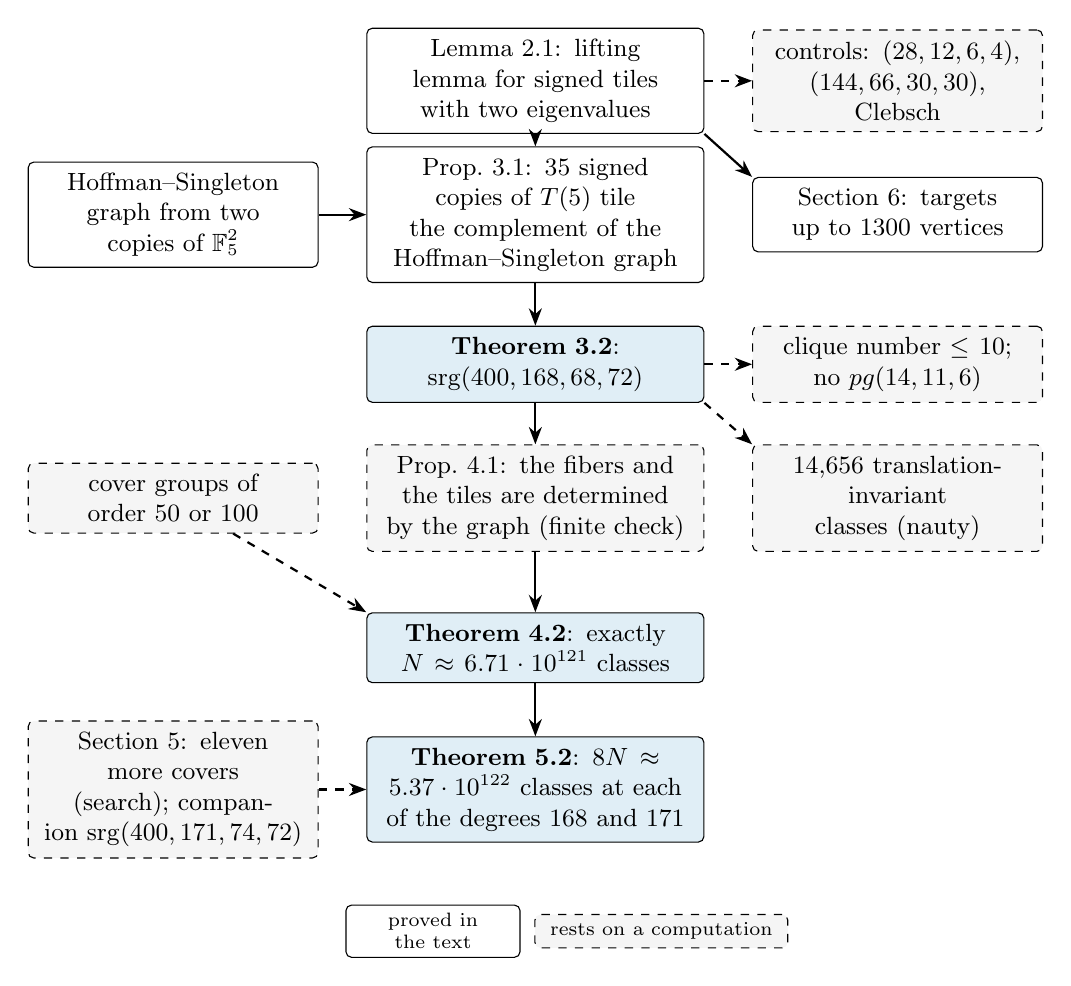
\begin{tikzpicture}[
  font=\small,
  box/.style={draw, rounded corners=2pt, align=center, text width=#1, inner sep=4pt, fill=white},
  box/.default=4.0cm,
  comp/.style={box=#1, dashed, fill=gray!8},
  comp/.default=3.4cm,
  arr/.style={-{Stealth[length=2.2mm]}, thick}]
% main column
\node[box] (lem) at (0,0) {Lemma 2.1: lifting lemma for signed tiles with two eigenvalues};
\node[box] (til) at (0,-1.7) {Prop.~3.1: $35$ signed copies of $T(5)$ tile the complement of the Hoffman--Singleton graph};
\node[box, fill=pA!12] (thm) at (0,-3.6) {\textbf{Theorem 3.2}: $\srg(400,168,68,72)$};
\node[comp=4.0cm] (rec) at (0,-5.3) {Prop.~4.1: the fibers and the tiles are determined by the graph (finite check)};
\node[box, fill=pA!12] (cnt) at (0,-7.2) {\textbf{Theorem 4.2}: exactly $N\approx6.71\cdot10^{121}$ classes};
% left column
\node[box=3.4cm] (hs) at (-4.6,-1.7) {Hoffman--Singleton graph from two copies of $\F_5^2$};
\node[comp] (cov) at (-4.6,-5.3) {cover groups of order $50$ or $100$};
\node[comp] (cv) at (-4.6,-9.0) {Section 5: eleven more covers (search); companion $\srg(400,171,74,72)$};
% right column
\node[comp] (ctl) at (4.6,0) {controls: $(28,12,6,4)$, $(144,66,30,30)$, Clebsch};
\node[comp] (ti) at (4.6,-5.3) {$14{,}656$ translation-invariant classes (nauty)};
\node[comp] (clq) at (4.6,-3.6) {clique number $\le10$; no $pg(14,11,6)$};
\node[box=3.4cm] (oth) at (4.6,-1.7) {Section 6: targets up to $1300$ vertices};
% arrows
\draw[arr] (lem) -- (til); \draw[arr] (til) -- (thm); \draw[arr] (thm) -- (rec); \draw[arr] (rec) -- (cnt);
\draw[arr] (hs) -- (til);
\node[box, fill=pA!12] (c12) at (0,-9.0) {\textbf{Theorem 5.2}: $8N\approx5.37\cdot10^{122}$ classes at each of the degrees $168$ and $171$};
\draw[arr] (cnt) -- (c12);
\draw[arr, dashed] (cv) -- (c12);
\draw[arr, dashed] (lem) -- (ctl);
\draw[arr] (lem.south east) -- (oth.north west);
\draw[arr, dashed] (cov) -- (cnt.north west);
\draw[arr, dashed] (thm.south east) -- (ti.north west);
\draw[arr, dashed] (thm) -- (clq);
% legend
\node[box=2.0cm, inner sep=3pt, font=\scriptsize] at (-1.3,-10.8) {proved in the text};
\node[comp=3.0cm, inner sep=3pt, font=\scriptsize] at (1.6,-10.8) {rests on a computation};
\end{tikzpicture}
}
\caption{How the results depend on each other. Solid boxes are proved in the text, and dashed boxes rest on a computation listed in Section~\ref{sec:data}.}
\label{fig:flow}
\end{figure}

\subsection*{Acknowledgments}
The co-Hoffman--Singleton cell graph, the eight-point slab construction and the signed $T(5)$ component type for this row are recorded in Anton Kova\v{l}'s search ledger~\cite{Kov26}, which left the case of a free $C_5\times C_5$ action on the cells unresolved. We thank him for sharing it.

\subsection*{Use of AI}
AI assistants were used for the search and verification programs and for a first draft of the text. GPT~6.2 Astra proposed the initial constructions. Claude Opus~5.5 audited and verified them and helped draft the first version of this note. The author has verified and finalized all results and text.

\begin{thebibliography}{9}
\bibitem{BrTab} A.~E.~Brouwer, Parameters of strongly regular graphs, \url{https://aeb.win.tue.nl/graphs/srg/srgtab.html}.
\bibitem{BR49} R.~H.~Bruck and H.~J.~Ryser, The nonexistence of certain finite projective planes, \emph{Canad. J. Math.} 1 (1949) 88--93.
\bibitem{Coo05} K.~Coolsaet, The uniqueness of the strongly regular graph srg(105,32,4,12), \emph{Bull. Belg. Math. Soc. Simon Stevin} 12 (2005) 707--718.
\bibitem{FDF02} D.~G.~Fon-Der-Flaass, New prolific constructions of strongly regular graphs, \emph{Adv. Geom.} 2 (2002) 301--306.
\bibitem{HS60} A.~J.~Hoffman and R.~R.~Singleton, On Moore graphs with diameters 2 and 3, \emph{IBM J. Res. Dev.} 4 (1960) 497--504.
\bibitem{Kov26} A.~Kova\v{l}, search ledger for open strongly regular graph parameters (hyperplane-slab template, row $(400,168,68,72)$), unpublished, 2026.
\bibitem{KovMO} A.~Kova\v{l}, Strongly regular graphs on 306, 400, 576, 784 and 1296 vertices from multi-orbit coset fusion and Bush-type Hadamard matrices, preprint, 2026, \url{https://doi.org/10.5281/zenodo.23296158}.
\bibitem{LTS89} C.~W.~H.~Lam, L.~Thiel and S.~Swiercz, The nonexistence of finite projective planes of order 10, \emph{Canad. J. Math.} 41 (1989) 1117--1123.
\bibitem{Muz07} M.~Muzychuk, A generalization of Wallis--Fon-Der-Flaass construction of strongly regular graphs, \emph{J. Algebraic Combin.} 25 (2007) 169--187.
\bibitem{P496} D.~Plummer, Strongly regular graphs with parameters $(496,231,102,112)$, note, 2026.
\bibitem{PT09} S.~E.~Payne and J.~A.~Thas, \emph{Finite Generalized Quadrangles}, 2nd ed., EMS, 2009.
\bibitem{Wal71} W.~D.~Wallis, Construction of strongly regular graphs using affine designs, \emph{Bull. Austral. Math. Soc.} 4 (1971) 41--49.
\end{thebibliography}

\end{document}
